\chapter{Redistribution Methods}
\label{sec:redist}

\inspire{My mind is like a racing engine, tearing itself to pieces because it is not connected up with the work for which it was built.}{Sherlock Holmes}
\vspace{0.5cm}


One final challenge similar to, but distinct from reading in data is managing data which has already been read into the R processes.  Throughout this chapter, we will be making reference to several particulars to the block-cyclic data type used for objects of
class \code{ddmatrix}.\index{Class!\code{ddmatrix}}
In particular, a working knowledge of the block-cyclic data structure and their relationship with BLACS~\index{Library!BLACS} contexts is most useful for the content to follow.  As such, the reader is \emph{strongly} encouraged to be familiar with the content of the \pkg{pbdDMAT} vignette before proceeding.

\section{Distributed Matrix Redistributions}
\label{sec:dmatredist}

\emph{Example:  Convert between different distributed matrix distributions.}

The demo command is
\begin{Command}
### At the shell prompt, run the demo with 4 processors by
### (Use Rscript.exe for windows system)
mpiexec -np 4 Rscript -e "demo(reblock,'pbdDEMO',ask=F,echo=F)"
\end{Command}

The distributed matrix class \code{ddmatrix}\index{Class!\code{ddmatrix}}
has two components which can be specified, and modified, by the user to 
drastically affect the composition of the distributed matrix.  In particular, 
these are the object's block-cyclic blocking factor \code{bldim}, and the 
BLACS~\index{Library!BLACS} communicator number \code{CTXT} which sets the 
2-dimensional processor grid. 

Thankfully, redistributing is a fairly simple process; though we would emphasize 
that \textbf{this is not free of cost}.  Reshaping data, especially at scale, 
can be much more expensive in total than even computation time.  That said, 
sometimes data must move.  It is better to get the job done slowly than to 
``take your ball and go home'' with no results.  But we caution that if 
redistribution can be avoided, then it should, at all costs.

There are several ways one can redistribute a \code{ddmatrix}.  To move the 
data to a block distribution, one can use the routines \code{as.rowblock()} and 
\code{as.colblock()} for 1-dimensional block distributions, and 
\code{as.block()} for a 2-dimensional block distribution.  Similarly, there are 
\code{as.rowcyclic()} and \code{as.colcyclic()} functions.  

Specifically, these methods take an object of class 
\code{ddmatrix}\index{Class!\code{ddmatrix}} as both an input and an output; 
i.e., and to emphasize the title of the chapter, this is not a method of 
\emph{distribution} but \emph{redistribution}.  The distribution details of 
the returned \code{ddmatrix} are according to the calling method.  For example, 
calling \code{as.block()} will return a 2-d block-cyclically distributed matrix 
which is also a 2-d block distributed matrix; see Chapter~\ref{chap:dmat} for 
information about this distinction.

\begin{figure}[ht]
        \centering
        \begin{subfigure}[b]{0.3\textwidth}
                \centering
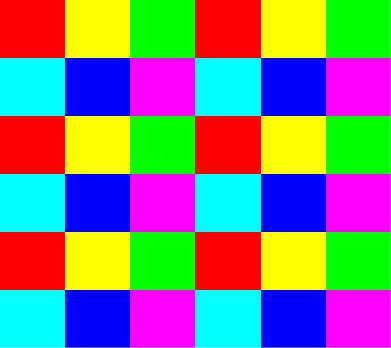
\includegraphics[height=5cm,width=\textwidth]{pbdDEMO-include/pics/bc}
                \caption{\code{as.blockcyclic()}}
        \end{subfigure}
        \hspace{.1cm}
        \begin{subfigure}[b]{0.3\textwidth}
                \centering

\includegraphics[height=5cm,width=\textwidth]{pbdDEMO-include/pics/block}
                \caption{\code{as.block()}}
        \end{subfigure}
        \hspace{.1cm}
        \begin{subfigure}[b]{0.3\textwidth}
                \centering

\includegraphics[height=5cm,width=\textwidth]{pbdDEMO-include/pics/rowblock}
                \caption{\code{as.rowblock()}}
        \end{subfigure}
\\[.3cm]
        \begin{subfigure}[b]{0.3\textwidth}

\includegraphics[height=5cm,width=\textwidth]{pbdDEMO-include/pics/colblock}
                \caption{\code{as.colblock()}}
        \end{subfigure}
        \hspace{.1cm}
        \begin{subfigure}[b]{0.3\textwidth}

\includegraphics[height=5cm,width=\textwidth]{pbdDEMO-include/pics/rowcyclic}
                \caption{\code{as.rowcyclic()}}
        \end{subfigure}
        \hspace{.1cm}
        \begin{subfigure}[b]{0.3\textwidth}

\includegraphics[height=5cm,width=\textwidth]{pbdDEMO-include/pics/colcyclic}
                \caption{\code{as.colcyclic()}}
        \end{subfigure}
        
        \caption{Matrix Redistribution Functions}
        \label{fig:redistplots}
\end{figure}

Figure~\ref{fig:redistplots} shows an 
example set of outputs for any \code{ddmatrix} input.  Here we assume that there 
are 6 processors, and in the block and block-cyclic cases, we are assuming that 
the processor grid (BLACS context) is a $2\times 3$ grid.

However, there is a much more general method available, namely 
\code{redistribute()}.  As the name implies, this method is for reshaping a 
block-cyclically distributed matrix of one kind to any another.  For example, if 
we have a distributed matrix \code{dx} and we wish to reshape the distributed 
matrix so that it now has blocking dimension \code{newbldim} and is distributed 
across BLACS~\index{Library!BLACS} context \code{newCTXT}, then I need merely 
call:

\begin{lstlisting}[language=rr]
dy <- redistribute(dx, bldim=newbldim, ICTXT=newCTXT)
\end{lstlisting}

Assuming the data is block cyclic of \emph{any} kind, including degenerate 
cases, we can convert it to a block cyclic format of any other kind we wish via 
this \code{redistribute()} function.  The only requirement is that the two 
different distributions have at least 1 processor in common, and so using the 
default BLACS~\index{Library!BLACS} contexts (0, 1, and 2) is always acceptable.




\section{Implicit Redistributions}
\label{sec:implicitredist}

There are several useful functions which apply to distributed matrices, but require a data redistribution as in Section~\ref{sec:redist}, whether the user realizes it or not.
\begin{table}[h]
\centering
\begin{tabular}{llll}\hline\hline
\textbf{Function} & \textbf{Example} & \textbf{Package} & \textbf{Effect}\\\hline
\code{`[`} & \code{dx[, -1]} & \pkg{pbdBASE} & Row/Column extraction and subsetting\\
\code{na.exclude()} & \code{na.exclude(dx)} & \pkg{pbdBASE} & Drop rows with \code{NA}'s\\
\code{apply()} & \code{apply(dx, 2, sd)} & \pkg{pbdDMAT} & Applies function to margin\\ \hline\hline
\end{tabular}
\caption[Implicit Data Redistributions]{Distributed Matrix Methods with Implicit Data Redistributions}
\label{tab:implicitredist}
\end{table}
These functions are listed in Table~\ref{tab:implicitredist}.  By default, 
these functions will re-distribute back to the original data distribution after 
having performed the initial (necessary) redistribution and performed the 
requested operations.  That is, by default, the problem of managing different 
data distributions is hidden from the user and entirely implicit.  However, 
there are advantages to becoming familiar with managing these data 
distributions, because each of these functions has the option to have 
redistribution directly managed.  Now, a data redistribution must occur to use 
these functions, but understanding which and why can help minimize the number of 
redistributions performed.

Many of the full details, such as \emph{why} the redistributions need occur in 
the first place, are outlined in the \pkg{pbdDMAT} vignette, but we provide a 
simple example here.  Suppose we have a distributed matrix \code{dx} distributed 
on the default grid (i.e., BLACS~\index{Library!BLACS} context 0) and we wish to 
drop the first column and then use the \code{apply()} function to extract the 
p-values, column-wise, of the result of running the Shapiro-Wilk normality test 
independently on the columns.  No one is claiming that this is a wise thing to 
do, but it is useful for the purpose of demonstration.

To achieve this, we could execute the following:

\begin{lstlisting}[language=rr,title=Implicit Redistributions]
dx <- dx[-1, ]

result <- apply(dx, MARGIN=2, FUN=function(col) shapiro.test(col)$p, reduce=TRUE)
\end{lstlisting}

In reality, underneath this is actually performing the following sequence of operations:

\begin{lstlisting}[language=rr,title=Implicit Redistributions]
dx <- redistribute(dx, ICTXT=2)
dx <- dx[, -1]
dx <- redistribute(dx, ICTXT=0)

dx <- redistribute(dx, ICTXT=2)
result <- apply(dx, MARGIN=2, FUN=function(col) shapiro.test(col)$p, reduce=TRUE)
\end{lstlisting}

Or suppose we wanted instead to drop the first column; then this is equivalent to

\begin{lstlisting}[language=rr,title=Implicit Redistributions]
dx <- redistribute(dx, ICTXT=1)
dx <- dx[, -1]
dx <- redistribute(dx, ICTXT=0)

dx <- redistribute(dx, ICTXT=2)
result <- apply(dx, MARGIN=2, FUN=function(col) shapiro.test(col)$p, reduce=TRUE)
\end{lstlisting}

The problem should be obvious.  However, thoroughly understanding the problem, 
we can easily manage the data redistributions using the \code{ICTXT=} option in 
these function.  So for example, we can minimize the redistributions to only the 
minimal necessary amount with the following:

\begin{lstlisting}[language=rr,title=Implicit Redistributions]
dx <- dx[, -1, ICTXT=2]

result <- apply(dx, MARGIN=2, FUN=function(col) shapiro.test(col)$p, reduce=TRUE)
\end{lstlisting}

This is equivalent to explicitly calling:

\begin{lstlisting}[language=rr,title=Implicit Redistributions]
dx <- redistribute(dx, ICTXT=2)
dx <- dx[, -1, ICTXT=2]

result <- apply(dx, MARGIN=2, FUN=function(col) shapiro.test(col)$p, reduce=TRUE)
\end{lstlisting}

This is clearly preferred.  For more details, see the relevant function documentation.




\section[Load Balance and Unload Balance]{Load Balance and Unload Balance}
\label{sec:lb_ub}

\emph{Example:  Load balancing (and unbalancing) distributed data.}

The demo command is
\begin{Command}
### At the shell prompt, run the demo with 4 processors by
### (Use Rscript.exe for windows system)
mpiexec -np 4 Rscript -e "demo(balance,'pbdDEMO',ask=F,echo=F)"
\end{Command}

Suppose we have an unbalanced, distributed input matrix \code{X.gbd}.  We can 
call \code{balance.info()} on this object to store some information about how to 
balance the data load across all processors.  This can be useful for tracking 
data movement, as well as for ``unbalancing'' later, if we so choose.  Next, we 
call
\code{load.balance()}~\index{Code!\code{load.balance()}}
to obtain a load-balanced object \code{new.X.gbd}.  We can also now undo this entire process and get back to \code{X.gbd} by calling
\code{unload.balance()}~\index{Code!\code{unload.balance()}} on \code{new.X.gbd}.


All together, the code looks something like:
\begin{Code}[title=R Code]
bal.info <- balance.info(X.gbd)
new.X.gbd <- load.balance(X.gbd, bal.info)
org.X.gbd <- unload.balance(new.X.gbd, bal.info)
\end{Code}

The details of this exchange are depicted in the example in Figure~\ref{fig:load_balance}.  Here, 
\code{X.gbd} is unbalanced, and \code{new.X.gbd} is a balanced version of \code{X.gbd}.

\begin{figure}[h]
\begin{center}
\begin{tabular}{ccc}
\code{X.gbd}(\code{org.X.gbd}) & & \code{new.X.gbd} \\

$
\left[
\begin{array}{ccc}
\color{p0}x_{1,1} & \color{p0}x_{1,2} & \color{p0}x_{1,3} \\ \hline
\color{p1}x_{2,1} & \color{p1}x_{2,2} & \color{p1}x_{2,3} \\
\color{p1}x_{3,1} & \color{p1}x_{3,2} & \color{p1}x_{3,3} \\ \hline
\color{p2}x_{4,1} & \color{p2}x_{4,2} & \color{p2}x_{4,3} \\
\color{p2}x_{5,1} & \color{p2}x_{5,2} & \color{p2}x_{5,3} \\
\color{p2}x_{6,1} & \color{p2}x_{6,2} & \color{p2}x_{6,3} \\ \hline
\color{p3}x_{7,1} & \color{p3}x_{7,2} & \color{p3}x_{7,3} \\
\color{p3}x_{8,1} & \color{p3}x_{8,2} & \color{p3}x_{8,3} \\
\color{p3}x_{9,1} & \color{p3}x_{9,2} & \color{p3}x_{9,3} \\
\color{p3}x_{10,1} & \color{p3}x_{10,2} & \color{p3}x_{10,3} \\
\end{array}
\right]
$

&

$
\begin{array}{c}
\mbox{\code{load.balance()}} \\
\longrightarrow \\
\hspace{0.5cm}\\
\longleftarrow \\
\mbox{\code{unload.balance()}} \\
\end{array}
$

&

$
\left[
\begin{array}{ccc}
\color{p0}x_{1,1} & \color{p0}x_{1,2} & \color{p0}x_{1,3} \\
\color{p0}x_{2,1} & \color{p0}x_{2,2} & \color{p0}x_{2,3} \\
\color{p0}x_{3,1} & \color{p0}x_{3,2} & \color{p0}x_{3,3} \\ \hline
\color{p1}x_{4,1} & \color{p1}x_{4,2} & \color{p1}x_{4,3} \\
\color{p1}x_{5,1} & \color{p1}x_{5,2} & \color{p1}x_{5,3} \\
\color{p1}x_{6,1} & \color{p1}x_{6,2} & \color{p1}x_{6,3} \\ \hline
\color{p2}x_{7,1} & \color{p2}x_{7,2} & \color{p2}x_{7,3} \\
\color{p2}x_{8,1} & \color{p2}x_{8,2} & \color{p2}x_{8,3} \\
\color{p2}x_{9,1} & \color{p2}x_{9,2} & \color{p2}x_{9,3} \\ \hline
\color{p3}x_{10,1} & \color{p3}x_{10,2} & \color{p3}x_{10,3} \\
\end{array}
\right]
$
\end{tabular}
\end{center}
\caption[Load Balancing/Unbalancing Data]{
Load Balancing/Unbalancing Data:  $\bX$ is distributed in
\code{X.gbd}(\code{org.X.gbd}) and \code{new.X.gbd}.
Both are distributed row-wise in 4 processors.  The colors represent processors {\color{p0}0},
{\color{p1}1}, {\color{p2}2}, and {\color{p3}3}, respectively.
}
\label{fig:load_balance}
\end{figure}
 

The function \code{balance.info()} is extremely useful, because it will return the information used to load balance the given data \code{X.gbd}.  The return of \code{balance.info()} is a list consisting of two data frames,
\code{send()} and \code{recv()}, as well as two vectors,
\code{N.allgbd} and \code{new.N.allgbd}.  

Here, \code{send} records the original processor rank and the destination processor rank of the unbalanced data (that which is to be transmitted by that processor).
The \code{load.balance()}\index{Code!\code{load.balance()}}
function uses this table to move the data via \pkg{pbdMPI}'s \code{isend()} function.
If any ``destination rank'' is not the ``original rank'', then the corresponding data row will be moved to the appropriate processor.  On the other hand, \code{recv} records the original processor rank and the destination rank of balanced data (that which is received by that processor).

The \code{N.allgbd} and \code{new.N.allgbd} objects both have length equal to the communicator containing all numbers of rows of \code{X.gbd} before and after the balancing, respectively. This is for double checking and avoiding a 0-row matrix issue.

For \code{unload.balance}, the process amounts to reversing \code{bal.info} and passing it to \code{load.balance}.

Finally, note that the ``balanced'' data is chosen to be balanced in a very particular way; it is arguably not ``balanced'', since 3 processors own 3 rows while 1 owns 1 row, and it is perhaps more balanced to have 2 processors own 3 rows and 2 own 2.  However, we make this choice for the reason that our ``balanced'' data will always be a certain kind of degenerate block-cyclic structure.  We will discuss this at length in the following section.




\section{Convert Between GBD and DMAT}
\label{sec:gbd_dmat}

\emph{Example:  Convert between GBD and DMAT formats.}

The demo command is
\begin{Command}
### At the shell prompt, run the demo with 4 processors by
### (Use Rscript.exe for windows system)
mpiexec -np 4 Rscript -e "demo(gbd_dmat,'pbdDEMO',ask=F,echo=F)"
\end{Command}

The final redistribution challenge we will present is taking an object in GBD format and putting it in the DMAT format.  More precisely, we assume the input object \code{X.gbd} is in GBD and convert the object into an object of
class \code{ddmatrix}\index{Class!\code{ddmatrix}}
which we will call \code{X.dmat}.


The Figure~\ref{fig:gbd_dmat} illustrates an example \code{X.gbd} and \code{X.dmat} conversion.  For full details about the block-cyclic data format used for
class \code{ddmatrix},\index{Class!\code{ddmatrix}}
see the \pkg{pbdDMAT} vignette.  

To perform such a redistribution, one simply needs to call:~\index{Code!\code{gbd2dmat()}}\index{Code!\code{dmat2gbd()}}
\begin{Code}[title=R Code]
X.dmat <- gbd2dmat(X.gbd)
\end{Code}
or
\begin{Code}[title=R Code]
X.gbd <- dmat2gbd(X.dmat)
\end{Code}
Here, the \code{gbd2dmat} function does the following:
\begin{enumerate}
\item Check number of columns of \code{X.gbd}.  All
      processors should be the same.
\item Row balance the GBD matrix as necessary via \code{load.balance()} as in Section~\ref{sec:lb_ub}.
\item Call construct a new ddmatrix object (via the \code{new()} constructor) on the balanced matrix,
      say \code{X.dmat}, in BLACS~\index{Library!BLACS} context 2 (\code{ICTXT = 2}).
\item Redistribute \code{X.dmat} to another BLACS context as needed 
      (default \code{ICTXT = 0}) via the \code{base.reblock()} function as in Section~\ref{sec:dmatredist}.
\end{enumerate}
Note that the \code{load.balance()} function, as used above, is legitimately necessary here.  Indeed, this function takes a collection of distributed data and converts it into a degenerate block cyclic distribution; namely, this places the data in block ``1-cycle'' format, distributed across an $n\times 1$ processor grid.  In the context of Figure~\ref{fig:gbd_dmat} (where the aforementioned process is implicit), this is akin to first moving the data into a distributed matrix format with \code{bldim=c(3,3)} and \code{CTXT=2}.  Finally, we can take this degenerate block-cyclic distribution and again to Figure~\ref{fig:gbd_dmat} as our motivating example, we convert the data balanced data so that it has \code{bldim=c(2,2)} and \code{CTXT=0}.

\begin{figure}
\begin{center}
\begin{tabular}{ccc}
\code{X.gbd} & & \code{X.dmat} \\

$
\left[
\begin{array}{ccc}
\color{p0}x_{1,1} & \color{p0}x_{1,2} & \color{p0}x_{1,3} \\ \hline
\color{p1}x_{2,1} & \color{p1}x_{2,2} & \color{p1}x_{2,3} \\
\color{p1}x_{3,1} & \color{p1}x_{3,2} & \color{p1}x_{3,3} \\ \hline
\color{p2}x_{4,1} & \color{p2}x_{4,2} & \color{p2}x_{4,3} \\
\color{p2}x_{5,1} & \color{p2}x_{5,2} & \color{p2}x_{5,3} \\
\color{p2}x_{6,1} & \color{p2}x_{6,2} & \color{p2}x_{6,3} \\ \hline
\color{p3}x_{7,1} & \color{p3}x_{7,2} & \color{p3}x_{7,3} \\
\color{p3}x_{8,1} & \color{p3}x_{8,2} & \color{p3}x_{8,3} \\
\color{p3}x_{9,1} & \color{p3}x_{9,2} & \color{p3}x_{9,3} \\
\color{p3}x_{10,1} & \color{p3}x_{10,2} & \color{p3}x_{10,3} \\
\end{array}
\right]
$

&

$
\begin{array}{c}
\mbox{\code{gbd2dmat}} \\
\longrightarrow \\
\hspace{0.5cm}\\
\longleftarrow \\
\mbox{\code{dmat2gbd}} \\
\end{array}
$

&

$
\left[
\begin{array}{cc|c}
\color{p0}x_{1,1} & \color{p0}x_{1,2} & \color{p1}x_{1,3} \\
\color{p0}x_{2,1} & \color{p0}x_{2,2} & \color{p1}x_{2,3} \\ \hline
\color{p2}x_{3,1} & \color{p2}x_{3,2} & \color{p3}x_{3,3} \\
\color{p2}x_{4,1} & \color{p2}x_{4,2} & \color{p3}x_{4,3} \\ \hline
\color{p0}x_{5,1} & \color{p0}x_{5,2} & \color{p1}x_{5,3} \\
\color{p0}x_{6,1} & \color{p0}x_{6,2} & \color{p1}x_{6,3} \\ \hline
\color{p2}x_{7,1} & \color{p2}x_{7,2} & \color{p3}x_{7,3} \\
\color{p2}x_{8,1} & \color{p2}x_{8,2} & \color{p3}x_{8,3} \\ \hline
\color{p0}x_{9,1} & \color{p0}x_{9,2} & \color{p1}x_{9,3} \\
\color{p0}x_{10,1} & \color{p0}x_{10,2} & \color{p1}x_{10,3} \\
\end{array}
\right]
$
\end{tabular}
\end{center}
\caption[Converting Between GBD and DMAT]{
Converting Between GBD and DMAT:  $\bX$ is distributed in
\code{X.gbd} and \code{X.dmat}.
Both are distributed in 4 processors
where colors represents processor {\color{p0}0},
{\color{p1}1}, {\color{p2}2}, and {\color{p3}3}.
Note that \code{X.dmat} is in block-cyclic format of
$2\times 2$ grid with $2\times 2$ block dimension.
}
\label{fig:gbd_dmat}
\end{figure}



\section{Exercises}
\label{sec:redist_exercise}

\begin{enumerate}[label=\thechapter-\arabic*]
\item
\label{ex:convert_row_column}
In the Sections~\ref{sec:lb_ub} and \ref{sec:gbd_dmat},
we have seen the load balance of GBD matrix
and the conversion between GBD and DMAT where GBD matrices \code{X.gbd}
are presumed in row-major as shown in
the Figures~\ref{fig:load_balance} and \ref{fig:gbd_dmat}.
Create new functions
\code{gbdr2gbdc()} and \code{gbdc2gbdr()} converting between
row-major and column-major by utilizing functions \code{gbd2dmat()}
and \code{dmat2gbd()} and changing their option \code{gbd.major}.

\item
The demo code \code{demo/gbd_dmat.r} of \pkg{pbdDEMO} has a GBD row-major
matrix \code{X.gbd}.\index{GBD row-major matrix}
Utilize the functions developed in the
Exercise~\ref{ex:convert_row_column}.
Convert \code{X.gbd} to a column-major matrix \code{new.X.gbdc}
by calling \code{gbdr2gbdc()}, then convert \code{new.X.gbdc} back to a
row-major matrix \code{new.X.gbdr} by calling \code{gbdc2gbdr()}.
Check if \code{new.X.gbdr} were the same as \code{X.gbd}.

\item
In \pkg{pbdDEMO}, there are some internal functions \code{demo.gbdr2dmat()},
\code{demo.gbdc2dmat()}, \code{demo.dmat2gbdr()}, and
\code{demo.dmat2gbdc()} which have similar implementations as the
functions \code{gbdr2gbdc()} and \code{gbdc2gbdr()} of the
Exercise~\ref{ex:convert_row_column}. Utilize these functions as templates.
Create a function \code{gbd2gbd()} with an argument \code{new.major} (1, 2)
for designated row- or column-majors.
Return warnings or errors if the input matrix is not convertible.

\item
\label{ex:nc4_gbdr}
The demo code \code{demo/nc4_gbdc.r} of \pkg{pbdDEMO} is an example utilizing
GBD column-major matrix \code{X.gbdc} \index{GBD column-major matrix}
and dumps the matrix into a NetCDF4
file. Adjust the code. Create a GBD row-major matrix \code{X.gbdr} and dump
the matrix to a new NetCDF4 file \code{nc4_gbdr.nc} by utilizing the function
\code{ncvar_put_gbd()} with option \code{gbd.major = 1}. Verify that all
\code{TREFHT} values of both \code{nc4_gbdc.nc} and \code{nc4_gbdr.nc}
are identical.
{\color{blue}Hint:
The local matrix of a GBD row- or column-major matrix is still
row-major as the default of \proglang{R}.
}

\item
The \code{load.balance()} and \code{unload.balance()} have a potential bug
when data size is small and can not fit into the desired block size of
a block-cyclic matrix. For instance, four processes in
a GBD row-major format with a matrix $5\times 1$. The two functions will
(un-) balance the data in $2\times 1$ in process 0, and $1\times 1$ in others.
If the desired block size is $2\time 1$, then the data should be
$2\times 1$ in processes 0 and 1, $1\times 1$ in process 2, and no
element for processor 3. Does any way to fix these two functions?

\end{enumerate}

